\documentclass[pdflatex,compress,mathserif]{beamer}

%\usetheme[dark,framenumber,totalframenumber]{ElektroITK}
\usetheme[darktitle,framenumber,totalframenumber]{ElektroITK}

\usepackage[utf8]{inputenc}
\usepackage[T1]{fontenc}
\usepackage{lmodern}
\usepackage[bahasai]{babel}
\usepackage{amsmath}
\usepackage{amsfonts}
\usepackage{amssymb}
\usepackage{graphicx}
\usepackage{multicol}
\usepackage{framed}
\usepackage{minted}

\definecolor{LightGray}{gray}{0.95}

\usefonttheme[onlymath]{serif}

\newcommand*{\Scale}[2][4]{\scalebox{#1}{$#2$}}%

\setbeamertemplate{caption}[numbered]

\title{METODE NUMERIK}
\subtitle{Turunan Numerik}

\author{Mifta Nur Farid}

\begin{document}

\maketitle

\section{Pengantar}

\begin{frame}{Pengantar}
    \begin{itemize}
        \item Sub-CPMK:\\ Mahasiswa mampu melakukan turunan numerik \textbf{(C3, P2, A2)}
    \end{itemize}
    \begin{itemize}
        \item Bahan kajian:
        \begin{enumerate}
            \item Metode finite difference
        \end{enumerate}
    \end{itemize}
\end{frame}

\begin{frame}{Finite difference}
    \begin{itemize}
        \item Metode finite difference digunakan untuk mencari turunan dari suatu persamaan atau data
        \item Caranya adalah dengan mengambil perbedaan dari nilai $y(x)$ terhadap perbedaan nilai $x$
        \item Jika perbedaan nilai $x$-nya sama maka $\Delta x$ umumnya dinotasikan dengan $h$ atau step-size
    \end{itemize}
\end{frame}

\begin{frame}{Finite difference}
    \begin{center}
        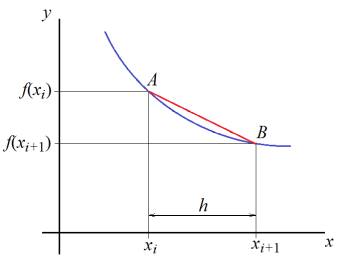
\includegraphics[width=0.8\linewidth]{img/img01}
    \end{center}
\end{frame}

\begin{frame}{Finite difference}
    \begin{itemize}
        \item Bentuk turunan yang paling sederhana bisa didapatkan dengan cara mencari kemiringan dari garis AB
        \item Kemiringan garis AB kira-kira sama dengan kemiringan tangen pada kurva di tengah antara $x_i$ dan $x_{i+1}$
        \item Semakin kecil step-size maka semakin akurat kemiringan yang didapatkan
        \item Urutan nilai kemiringan ini akan menghasilkan perkiraan turunan pertama dari data yang diberikan.
    \end{itemize}
\end{frame}


\begin{frame}{Finite difference}
    \begin{itemize}
        \item Secara teoritis, pendekatan finite difference berasal dari ekspansi deret Taylor $f(x)$. Ekspansi dari $f(x_{i+1})$ dapat ditulis sebagai berikut:
        $$ f(x_{i+1}) = f(x_i) + f'(x_i)h + \frac{f''(x_i)}{2!}h^2 + \frac{f'''(x_i)}{3!}h^3 + \cdots $$ maka
        $$ f'(x_i) = \frac{f(x_{i+1}) - f(x_i)}{h} - \frac{f''(x_i)}{2!}h^2 - \frac{f'''(x_i)}{3!}h^3 + \cdots $$
    \end{itemize}
\end{frame}

\begin{frame}{Finite difference}
    \begin{itemize}
        \item Dengan mengabaikan suku-suku yang mengandung turunan kedua dan yang lebih tinggi, persamaan:
        $$ f'(x_i) = \frac{f(x_{i+1}) - f(x_i)}{h} - \frac{f''(x_i)}{2!}h^2 - \frac{f'''(x_i)}{3!}h^3 + \cdots $$
        menjadi
        $$ f'(x_i) = \frac{f(x_{i+1}) - f(x_i)}{h} + O(h) $$
        \item Persamaan di atas disebut sebagai persamaan forward difference, karena titik kedua setelah $x_i$ dipilih di arah positif dari sumbu-x.
        \item Bentuk $O(h)$ menunjukkan error yang dihasilkan dari pemotongan yang dilakukan
    \end{itemize}
\end{frame}

\begin{frame}{Forward finite differences}
    \begin{align*}
        f'(x_i) &= \frac{f(x_{i+1}) - f(x_i)}{h}\\
        f''(x_i) &= \frac{f(x_{i+2}) - 2f(x_{i+1}) + f(x_i)}{h^2}\\
        f'''(x_i) &= \frac{f(x_{i+3}) - 3f(x_{i+2}) + 3f(x_{i+1}) - f(x_i)}{h^3}\\
        f''''(x_i) &= \frac{f(x_{i+4}) - 4f(x_{i+3}) + 6f(x_{i+2}) - 4f(x_{i+1}) + f(x_i)}{h^4}\\
    \end{align*}
\end{frame}

\begin{frame}{Central finite differences}
    \begin{align*}
        f'(x_i) &= \frac{f(x_{i+1}) - f(x_{i-1})}{2h}\\
        f''(x_i) &= \frac{f(x_{i+1}) - 2f(x_{i}) + f(x_{i-1})}{h^2}\\
        f'''(x_i) &= \frac{f(x_{i+2}) - 2f(x_{i+1}) + 2f(x_{i-1}) - f(x_{i-2})}{2h^3}\\
        f''''(x_i) &= \frac{f(x_{i+2}) - 4f(x_{i+1}) + 6f(x_{i}) - 4f(x_{i-1}) + f(x_{i-2})}{h^4}\\
    \end{align*}
\end{frame}

\begin{frame}{Backward finite differences}
    \begin{align*}
        f'(x_i) &= \frac{f(x_{i}) - f(x_{i-1})}{h}\\
        f''(x_i) &= \frac{f(x_i) - 2f(x_{i-1}) + f(x_{i-2})}{h^2}\\
        f'''(x_i) &= \frac{f(x_i) - 3f(x_{i-1}) + 3f(x_{i-2}) - f(x_{i-3})}{h^3}\\
        f''''(x_i) &= \frac{f(x_i) - 4f(x_{i-1}) + 6f(x_{i-2}) - 4f(x_{i-3}) + f(x_{i-4})}{h^4}\\
    \end{align*}
\end{frame}


\end{document}
